\section{Conclusion}
\label{sec:conclusion}

In conclusion, the review of this paper has been a great opportunity to dive into the world of neural rendering and understand the challenges of point based neural rendering.

\noindent I have implemented two major items: 
\begin{itemize}
    \item A script to render calibrated scenes which are ready for neural rendering (with perfect normals, perfect point cloud position and camera poses). 
    \item A pytorch implementation of point projections with the fuzzy depth test (which was satisfying and fast enough to perform live inference)
\end{itemize}
I was therefore able to train a simple multiscale decoder CNN jointly with point pseudo colors on simple calibrated scene.

\noindent I have pointed out:
\begin{itemize}
    \item a minor criticism regarding all tricks deployed to model the camera pipeline instead of truly questioning the relevance of benchmarks on the Tanks and Temple dataset. 
    \item a limitation regarding handling view dependent effects which is not a problem in NERF.
\end{itemize}

\noindent The amount of work spent by the authors to make their method work very fast on large scale point clouds is tremendous. The crafstmanship of the computer graphics research community is very inspiring.



\begin{figure}[H]
    \centering
    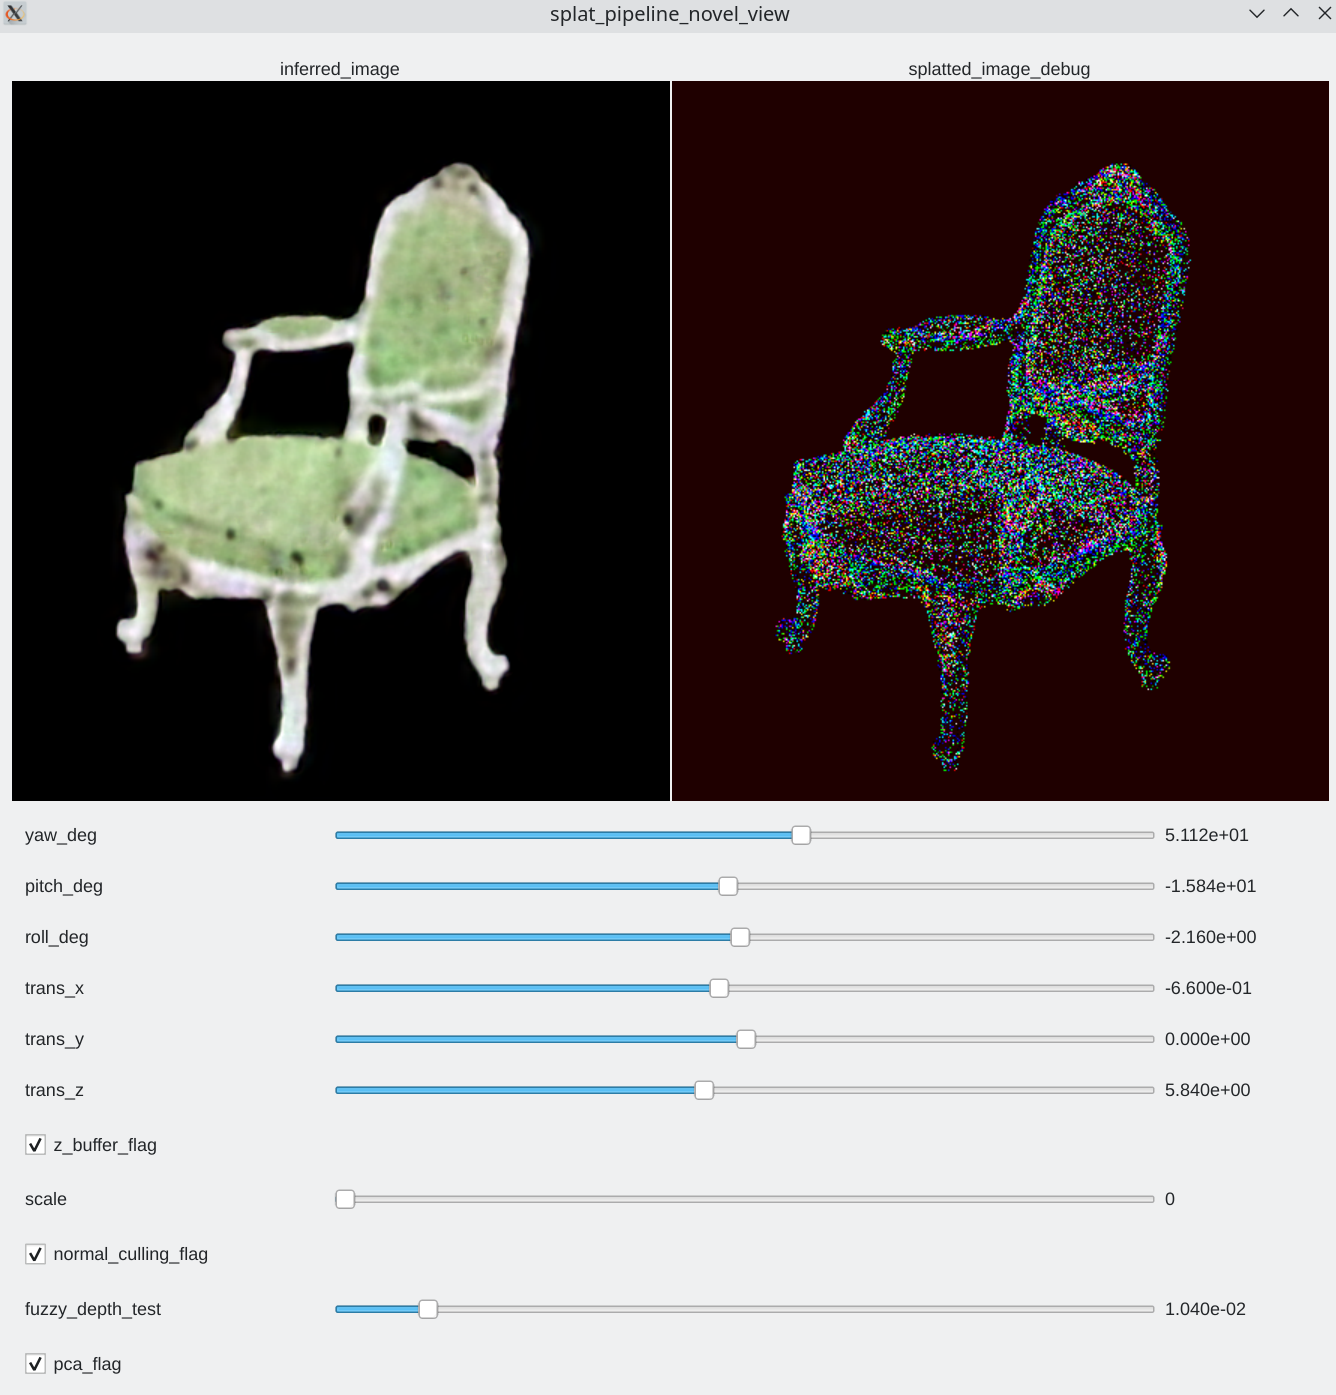
\includegraphics[width=0.4\textwidth]{figures/inference_live.png}
    \caption{Live inference, the user can move the camera around the scene and see the novel view rendered in real time. On the right side we visualize the projected pseudo colored point cloud of dimension 8 using a Principal Component Analyzis.}
    \label{fig:live_inference}
\end{figure}